\section{【背景】内存管理:理解保护模式和分段机制}\label{ux80ccux666fux5185ux5b58ux7ba1ux7406ux7406ux89e3ux4fddux62a4ux6a21ux5f0fux548cux5206ux6bb5ux673aux5236}

为何要了解Intel 80386的保护模式和分段机制?首先,我们知道Intel
80386只有在进入保护模式后,才能充分发挥其强大的功能,提供更好的保护机制和更大的寻址空间,否则仅仅是一个快速的8086而已。没有一定的保护机制,任何一个应用软件都可以任意访问所有的计算机资源,这样也就无从谈起操作系统设计了。且Intel
80386的分段机制一直存在,无法屏蔽或避免。其次,在我们的bootloader设计中,涉及到了从实模式到保护模式的处理,我们的操作系统功能(比如分页机制)是建立在Intel
80386的保护模式上来设计的。如果我们不了解保护模式和分段机制,则我们面向Intel
80386体系结构的操作系统设计实际上是建立在一个空中楼阁之上。

\subsection{实模式}\label{ux5b9eux6a21ux5f0f}

80386的实模式是为了与8086处理器兼容而设置的。在实模式下,80386处理器就相当于一个快速的8086处理器。80386处理器被复位或加电的时候以实模式启动。这时候处理器中的各寄存器以实模式的初始化值工作。80386处理器在实模式下的存储器寻址方式和8086基本一致,由段寄存器的内容乘以16作为基地址,加上段内的偏移地址形成最终的物理地址,这时候它的32位地址线只使用了低20位,即可访问1MB的物理地址空间。在实模式下,80386处理器不能对内存进行分页机制的管理,所以指令寻址的地址就是内存中实际的物理地址。在实模式下,所有的段都是可以读、写和执行的。实模式下80386不支持优先级,所有的指令相当于工作在特权级(即优先级0),所以它可以执行所有特权指令,包括读写控制寄存器CR0等。这实际上使得在实模式下不太可能设计一个有保护能力的操作系统。实模式下不支持硬件上的多任务切换。实模式下的中断处理方式和8086处理器相同,也用中断向量表来定位中断服务程序地址。中断向量表的结构也和8086处理器一样,每4个字节组成一个中断向量,其中包括两个字节的段地址和两个字节的偏移地址。应用程序可以任意修改中断向量表的内容,使得计算机系统容易受到病毒、木马等的攻击,整个计算机系统的安全性无法得到保证。

\textbf{【历史:寻址空间:A20地址线与处理器向下兼容】}

Intel早期的8086
CPU提供了20根地址线,可寻址空间范围即0\textsubscript{2\^{}20(00000H}FFFFFH)的
1MB内存空间。但8086的数据处理位为16位,无法直接寻址1MB内存空间,所以8086提供了段地址加偏移地址的地址转换机制,就是我们常见的''段地址(16位):偏移地址(16位或有效地址)'',实际的计算方法为:''段地址*0x10H+偏移地址'',作为段地址的数据是放在段寄存器中的(16位),而作为位偏移地址的数据则是通过8086提供的寻址方式来计算而来的(16位)。而``段值:偏移''这种表示法能够表示的最大内存为0x10FFEEH(即0xFFFF0H~+~0xFFFFH),所以当寻址到超过1MB的内存时,会发生``回卷''(不会发生异常)。但下一代的基于Intel
80286 CPU的PC AT计算机系统提供了24根地址线,这样CPU的寻址范围变为
2\^{}24=16M,同时也提供了保护模式,可以访问到1MB以上的内存了,此时如果遇到``寻址超过1MB''的情况,系统不会再``回卷''了,这就造成了向下不兼容。为了保持完全的向下兼容性,IBM决定在PC
AT计算机系统上加个硬件逻辑,来模仿以上的回绕特征。他们的方法就是把A20地址线控制和键盘控制器的一个输出进行AND操作,这样来控制A20地址线的打开(使能)和关闭(屏蔽,禁止)。一开始时A20地址线控制是被屏蔽的(总为0),直到系统软件通过一定的I/O操作去打开它(参看bootloader的bootasm.S文件)。
当A20
地址线控制禁止时,则程序就像在8086中运行,1MB以上的地是不可访问的。在保护模式下A20地址线控制是要打开的。为了使能所有地址位的寻址能力,必须向键盘控制器8042发送一个命令。键盘控制器8042将会将它的的某个输出引脚的输出置高电平,作为
A20 地址线控制的输入。一旦设置成功之后,内存将不会再被绕回(memory
wrapping),这样我们就可以寻址intel 80286 CPU支持的16M
内存空间,或者是寻址intel 80386 以上级别CPU支持的所有 4G内存空间了。
8042键盘控制器的I/O端口是0x60~0x6f,实际上IBM
PC/AT使用的只有0x60和0x64两个端口(0x61、0x62和0x63用于与XT兼容目的)。8042通过这些端口给键盘控制器或键盘发送命令或读取状态。输出端口P2用于特定目的。位0(P20引脚)用于实现CPU复位操作,位1(P21引脚)用户控制A20信号线的开启与否。系统向输入缓冲(端口0x64)写入一个字节,即发送一个键盘控制器命令。可以带一个参数。参数是通过0x60端口发送的。
命令的返回值也从端口 0x60去读。
在proj1的bootasm.S中,``seta20.1''标号和``seta20.2''标号后的汇编代码即是用来完成A20地址线控制打开工作的。

\subsection{保护模式概述}\label{ux4fddux62a4ux6a21ux5f0fux6982ux8ff0}

简单地说,通过保护模式,可以把虚拟地址空间映射到不同的物理地址空间,且在超出预设的空间范围会报错(一种保护机制的体现),且可以保证处于低特权级的代码无法访问搞特权级的数据(另外一种保护机制的体现)。
只有在保护模式下,80386的全部32位地址才能有效,可寻址高达4G字节的线性地址空间和物理地址空间,可访问64TB(有2\textsuperscript{14个段,每个段最大空间为2}32字节)的虚拟地址空间,可采用分段存储管理机制和分页存储管理机制。这不仅为存储共享和保护提供了硬件支持,而且为实现虚拟存储提供了硬件支持。通过提供4个特权级和完善的特权检查机制,既能实现资源共享又能保证代码数据的安全及任务隔离。
在保护模式下,特权级总共有4个,编号从0(最高特权)到3(最低特权)。有3种主要的资源受到保护:内存,I/O地址空间以及执行特殊机器指令的能力。在任一时刻,intel
80386
CPU都是在一个特定的特权级下运行的,从而决定了代码可以做什么,不可以做什么。这些特权级经常被称为为保护环(protection
ring),最内的环(ring 0)对应于最高特权0,最外面的环(ring
3)一般给应用程序使用,对应最低特权3。在ucore中,CPU只用到其中的2个特权级:0(内核态)和3(用户态)。在保护模式下,我们可以通过查看CS寄存器的最低两位来了解当前正在运行的处理器是处于哪个特权级。

\subsection{分段机制的地址转换}\label{ux5206ux6bb5ux673aux5236ux7684ux5730ux5740ux8f6cux6362}

intel 80386
CPU提供了分段机制和分页机制两种内存管理方式,在当前计算机系统中是否需要这两种机制共存没有一个明确的答案,二者有它们各自独特的功能。在intel
80386
CPU中,只要进入保护模式,必然需要启动分段机制,且一直存在下去(分页不一定要一直存在),所以我们需要了解分段机制的原理。分段机制体现了内存中不同地址的一种转换/映射方式,即程序员编程所使用的地址(逻辑地址)和实际计算机中的物理地址需要通过分段机制来建立映射关系。分段机制将内存划分成以起始地址和长度限制这两个参数表示的内存块,这些内存块就称之为段(Segment)。编译器把源程序编译成执行程序时用到的代码段、数据段、堆和栈等概念在这里可以与段联系起来,二者在含义上是一致的。从操作系统原理上看,编译器实际上采用了基于分段的虚存管理方式来生成执行程序的,即应用程序员看到的逻辑地址和位于计算机上的物理地址之间有映射关系,二者可以是不同的。当然,后续章节中,我们还将介绍分页机制,即另一种使用更加广泛的地址转换/映射方式,这是操作系统实现虚存管理的重要基础。
简单地说,当CPU执行一条访存指令时(一个具体的指令),基于分段模式的具体硬件操作过程如下:

\begin{enumerate}
\def\labelenumi{\arabic{enumi}.}
\item
  根据指令的内容确定应该使用的段寄存器,比如取内存指令的内存地址所对应的数据段寄存器为DS;
\item
  根据段寄存器DS的值作为选择子,以此选择子值为索引,在段描述符表(可理解为一个大数组)找到索引指向的段描述符(可理解为数组中的元素);
\item
  在段描述符中取出基地址域(段的起始地址)和地址范围域(段的长度)的值;
\item
  将指令内容确定的地址偏移,与地址范围域的值比较,确保地址偏移小于地址范围,这样是为了确保地址范围不会跨出段的范围;(第一层保护)
\item
  根据指令的性质(当前指令的CS值的低两位)确定当前指令的特权级,需要高于当前指令访问的数据段的特权级;(第二层保护);
\item
  根据指令的性质(指令是做读还是写操作),需要当前指令访问的数据段可读或可写;(第三层保护)
\item
  将DS指向的段描述符中基地址域的值加上指令内容中指定的访存地址段内偏移值,形成实际的物理地址(实现地址转换),发到数据地址总线上,到物理内存中寻址,并取回该地址对应的数据内容。
  分段机制涉及4个关键内容:逻辑地址(Logical
  Address,应用程序员看到的地址,在操作系统原理上称为虚拟地址,以后提到虚拟地址就是指逻辑地址)、物理地址(Physical
  Address,
  实际的物理内存地址)、段描述符表(包含多个段描述符的``数组'')、段描述符(描述段的属性,及段描述符表这个``数组''中的``数组元素'')、段选择子(即段寄存器中的值,用于定位段描述符表中段描述符表项的索引)。
  虚拟地址到物理地址的转换主要分以下两步:
\item
  分段地址转换:CPU把虚拟地址(由段选择子selector和段偏移offset组成)中的段选择子值作为段描述符表的索引,找到表中对应的段描述符,然后把段描述符中保存的段基址加上段偏移值,形成线性地址(Linear
  Address,在操作系统原理上没有直接对应的描述,在没有启动分页机制的情况下,可认为就是物理地址;如果启动了分页机制,则可理解为第二级虚拟地址)。如果不启动分页存储管理机制,则线性地址等于物理地址。
\item
  分页地址转换,这一步中把线性地址转换为物理地址。(注意:这一步是可选的,由操作系统决定是否需要。在后续试验中会涉及。)
  上述转换过程对于应用程序员来说是不可见的。线性地址空间由一维的线性地址构成,在分段机制下的线性地址空间和物理地址空间对等。线性地址32位长,线性地址空间容量为4G字节。分段机制中虚拟地址到线性地址转换转换的基本过程如下图所示。
\end{enumerate}

%\begin{figure}[htbp]
%\centering
%
\includegraphics{figures/3.15.1.png}
%\caption{3.15.1}
%\end{figure}

图1 分段机制中虚拟地址到线性地址转换转换基本过程

分段存储管理机制需要在启动保护模式的前提下建立。从上图可以看出,为了使得分段存储管理机制正常运行,需要在启动保护模式前建立好段描述符和段描述符表(参看bootasm.S中的``lgdt
gdtdesc''语句和gdt标号/gdtdesc标号下的数据结构)。

\subsubsection{段选择子}\label{ux6bb5ux9009ux62e9ux5b50}

\textbf{段选择子}是用来选择哪个描述符表和在该表中索引哪一个描述符的。选择子可以做为指针变量的一部分,从而对应用程序员是可见的,但是一般是由编译器(gcc)和链接工具(ld)来设置的。段选择子的内容一般放在段寄存器中。选择子的格式如下图所示:

%\begin{figure}[htbp]
%\centering
%
\includegraphics{figures/3.15.2.png}
%\caption{3.15.2}
%\end{figure}

图2 段选择子结构

\textbf{索引(Index)}:在描述符表中从8192个描述符中选择一个描述符。处理器自动将这个索引值乘以8(描述符的长度),再加上描述符表的基址来索引描述符表,从而选出一个合适的描述符。

\textbf{表指示位(Table
Indicator,TI)}:选择应该访问哪一个描述符表。0代表应该访问全局描述符表(GDT);1代表应该访问局部描述符表(LDT)。LDT在实验中没有涉及。

\textbf{请求特权级(Requested Privilege
Level,RPL)}:用于段级的保护机制,比如,段选择子是CS,则这两位表示当前执行指令的处理器所处的特权级的值,从而你可以了解到当前处理器是处于用户态(Ring
3)还是内核态(Ring 0)。在后续试验中会进一步讲解。

\subsubsection{段描述符}\label{ux6bb5ux63cfux8ff0ux7b26}

在分段存储管理机制的保护模式下,每个段由如下三个参数进行定义:段基地址(Base
Address)、段界限(Limit)和段属性(Attributes)。

\textbf{段基地址}:即线性地址空间中段的起始地址。在80386保护模式下,段基地址长32位。因为基地址长度与寻址地址的长度相同,所以任何一个段都可以从32位线性地址空间中的任何一个字节开始,而不象实方式下规定的边界必须被16整除。
在实验中,一般都简化了段机制的使用,把所有段的段基地址设置为0。

\textbf{段界限}:规定段的大小。在80386保护模式下,段界限用20位表示,而且段界限可以是以单字节为最小单位或以4K字节为最小单位。在实验中,一般都简化了段机制的使用,把所有段的段界限设置为0xFFFFF,以4K字节为最小单位,即段的界限为4GB;

\textbf{类型(TYPE)}:用于区别不同类型的描述符。可表示所描述的段是代码段还是数据段,所描述的段是否可读/写/执行,段的扩展方向等。
\textbf{描述符特权级(Descriptor Privilege
Level)(DPL)}:用来实现保护机制。 \textbf{段存在位(Segment-Present
bit)}:如果这一位为0,则此描述符为非法的,不能被用来实现地址转换。如果一个非法描述符被加载进一个段寄存器,处理器会立即产生异常。图2显示了当存在位为0时,描述符的格式。操作系统可以任意的使用被标识为可用(AVAILABLE)的位。
\textbf{已访问位(Accessed
bit)}:当处理器访问该段(当一个指向该段描述符的选择子被加载进一个段寄存器)时,将自动设置访问位。操作系统可清除该位。
上述表示段的属性的参数通过段描述符(Segment
Descriptor)来表示,一个段描述符占8字节。段描述符的结构如下图所示:

%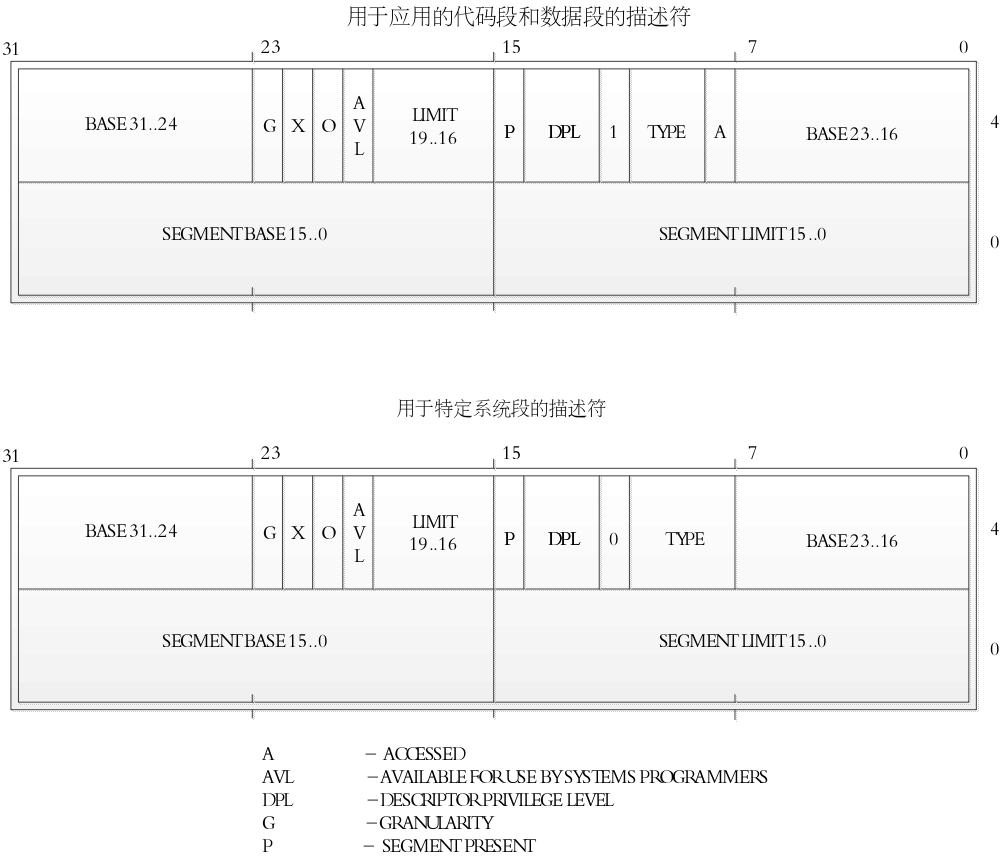
\includegraphics{figures/3.15.3.png} 

图2 段描述符结构

\subsubsection{全局描述符表}\label{ux5168ux5c40ux63cfux8ff0ux7b26ux8868}

全局描述符表的是一个保存多个段描述符的``数组'',其起始地址保存在全局描述符表寄存器GDTR中。GDTR长48位,其中高32位为基地址,低16位为段界限。由于GDT
不能用GDT本身之内的描述符进行描述定义,所以采用GDTR寄存器来表示GDT这一特殊的系统段。注意,全部描述符表中第一个段描述符设定为空段描述符。GDTR中的段界限以字节为单位。对于含有N个描述符的描述符表的段描述符实际所占空间通常可设为8\emph{N,若起始地址为gdt\_base,则结束地址为gdt\_base+8}N-1。可参考proj1中的bootasm.S中的gdt标号和gdtdesc标号下的内容,以及lgdt指令的操作数。
全局描述符表的第一项是不能被CPU使用,所以当一个段选择子的索引(Index)部分和表指示位(Table
Indicator)都为0的时(即段选择子指向全局描述符表的第一项时),可以当做一个空的选择子。当一个段寄存器被加载一个空选择子时,处理器并不会产生一个异常。但是,当用一个空选择子去访问内存时,则会产生异常。在proj1的实验中,值设置了三个段描述符,即NULL段、TEXT段和DATA段(都是4GB的访问范围)。

\subsection{分段机制的系统寄存器}\label{ux5206ux6bb5ux673aux5236ux7684ux7cfbux7edfux5bc4ux5b58ux5668}

80386
有4个寄存器来寻址描述发表等系统数据结构,用来实现段式内存管理。内存管理寄存器包括:

\begin{itemize}
\item
  全局描述符表寄存器 (Global Descriptor Table Register,GDTR
  ):指向全局段描述符表 GDT
\item
  局部描述符表寄存器 (Local Descriptor Table
  Register,LDTR):指向局部段描述符表 LDT~(目前用不上)
\item
  中断门描述符表寄存器 (Interrupt Descriptor Table
  Register,IDTR):指向一张包含中断处理子程序入口点的表(IDT)~
\item
  任务寄存器 (Task
  Register,TR):这个寄存器指向当前任务信息存放处,这些信息是处理器进行任务切换所需要的。(目前用不上)
  80386有四个32位的控制寄存器,分别命名位CR0、CR1、CR2和CR3。CR0包含指示处理器工作方式、启用和禁止分页管理机制、控制浮点协处理器操作的控制位。具体描述如下:
\item
  PE(保护模式允许 Protection Enable,比特位 0):设置PE
  将让处理器工作在保护模式下。复位PE将返回到实模式工作。
\item
  PG(分页允许 Paging, 比特位 31): PG
  指明处理器是否通过页表来转换线性地址到物理地址。在后续试验中将讲述如何设置PG位。
  CR0中的位5\textasciitilde{}位30是保留位,这些位的值必须为0。CR2及CR3由分页管理机制使用,将在后续试验中讲述。在80386中不能使用CR1,否则会引起无效指令操作异常。
\end{itemize}
